The Pinball domain of \cite{Konidaris2009} was chosen to better understand the practical implications of the options construction algorithm presented in the last chapter. This environment consists in arbitrarily shaped obstacles laid out on the plane and among which an agent must learn to navigate a ball to the target (figure \ref{fig:pinball}). The agent has access to four primitive discrete actions which increase or decrease the velocity of the ball in the $x$ and $y$ directions as well as a fifth \textit{null} action. Collisions with the obstacles are elastic and a drag coefficient of 0.995 effectively stops ball movements after a finite number of steps when the null action is chosen repeatedly. Each thrust action incurs a penaly of -5 while taking no action costs -1. The episode terminates with +10000 reward when the agent reaches  the target. A four-dimensional continuous observation vector $[ x, y, \dot{x}, \dot{y}]$ is available to the agent at every time step and is prone to sharp discontinuities. While the pinball environment as presented originally in \cite{Konidaris2009} is purely deterministic, normal noise with standard deviation $\sigma = 0.03$ was added exactly as in \cite{Tamar2013}. 

\begin{figure}
\centering
\subbottom[Pinball]{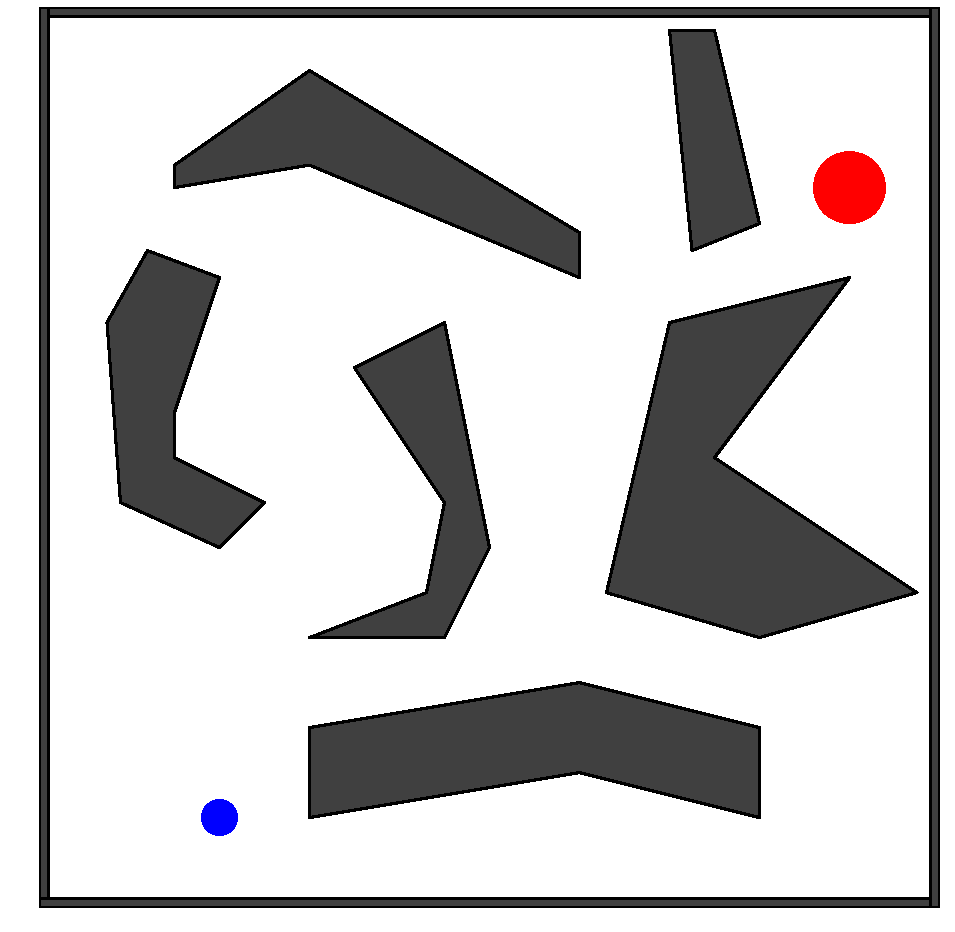
\includegraphics[width=0.32\textwidth]{fig/pinball.pdf}\label{fig:pinball}}%
\subbottom[Graph construction and pruning]{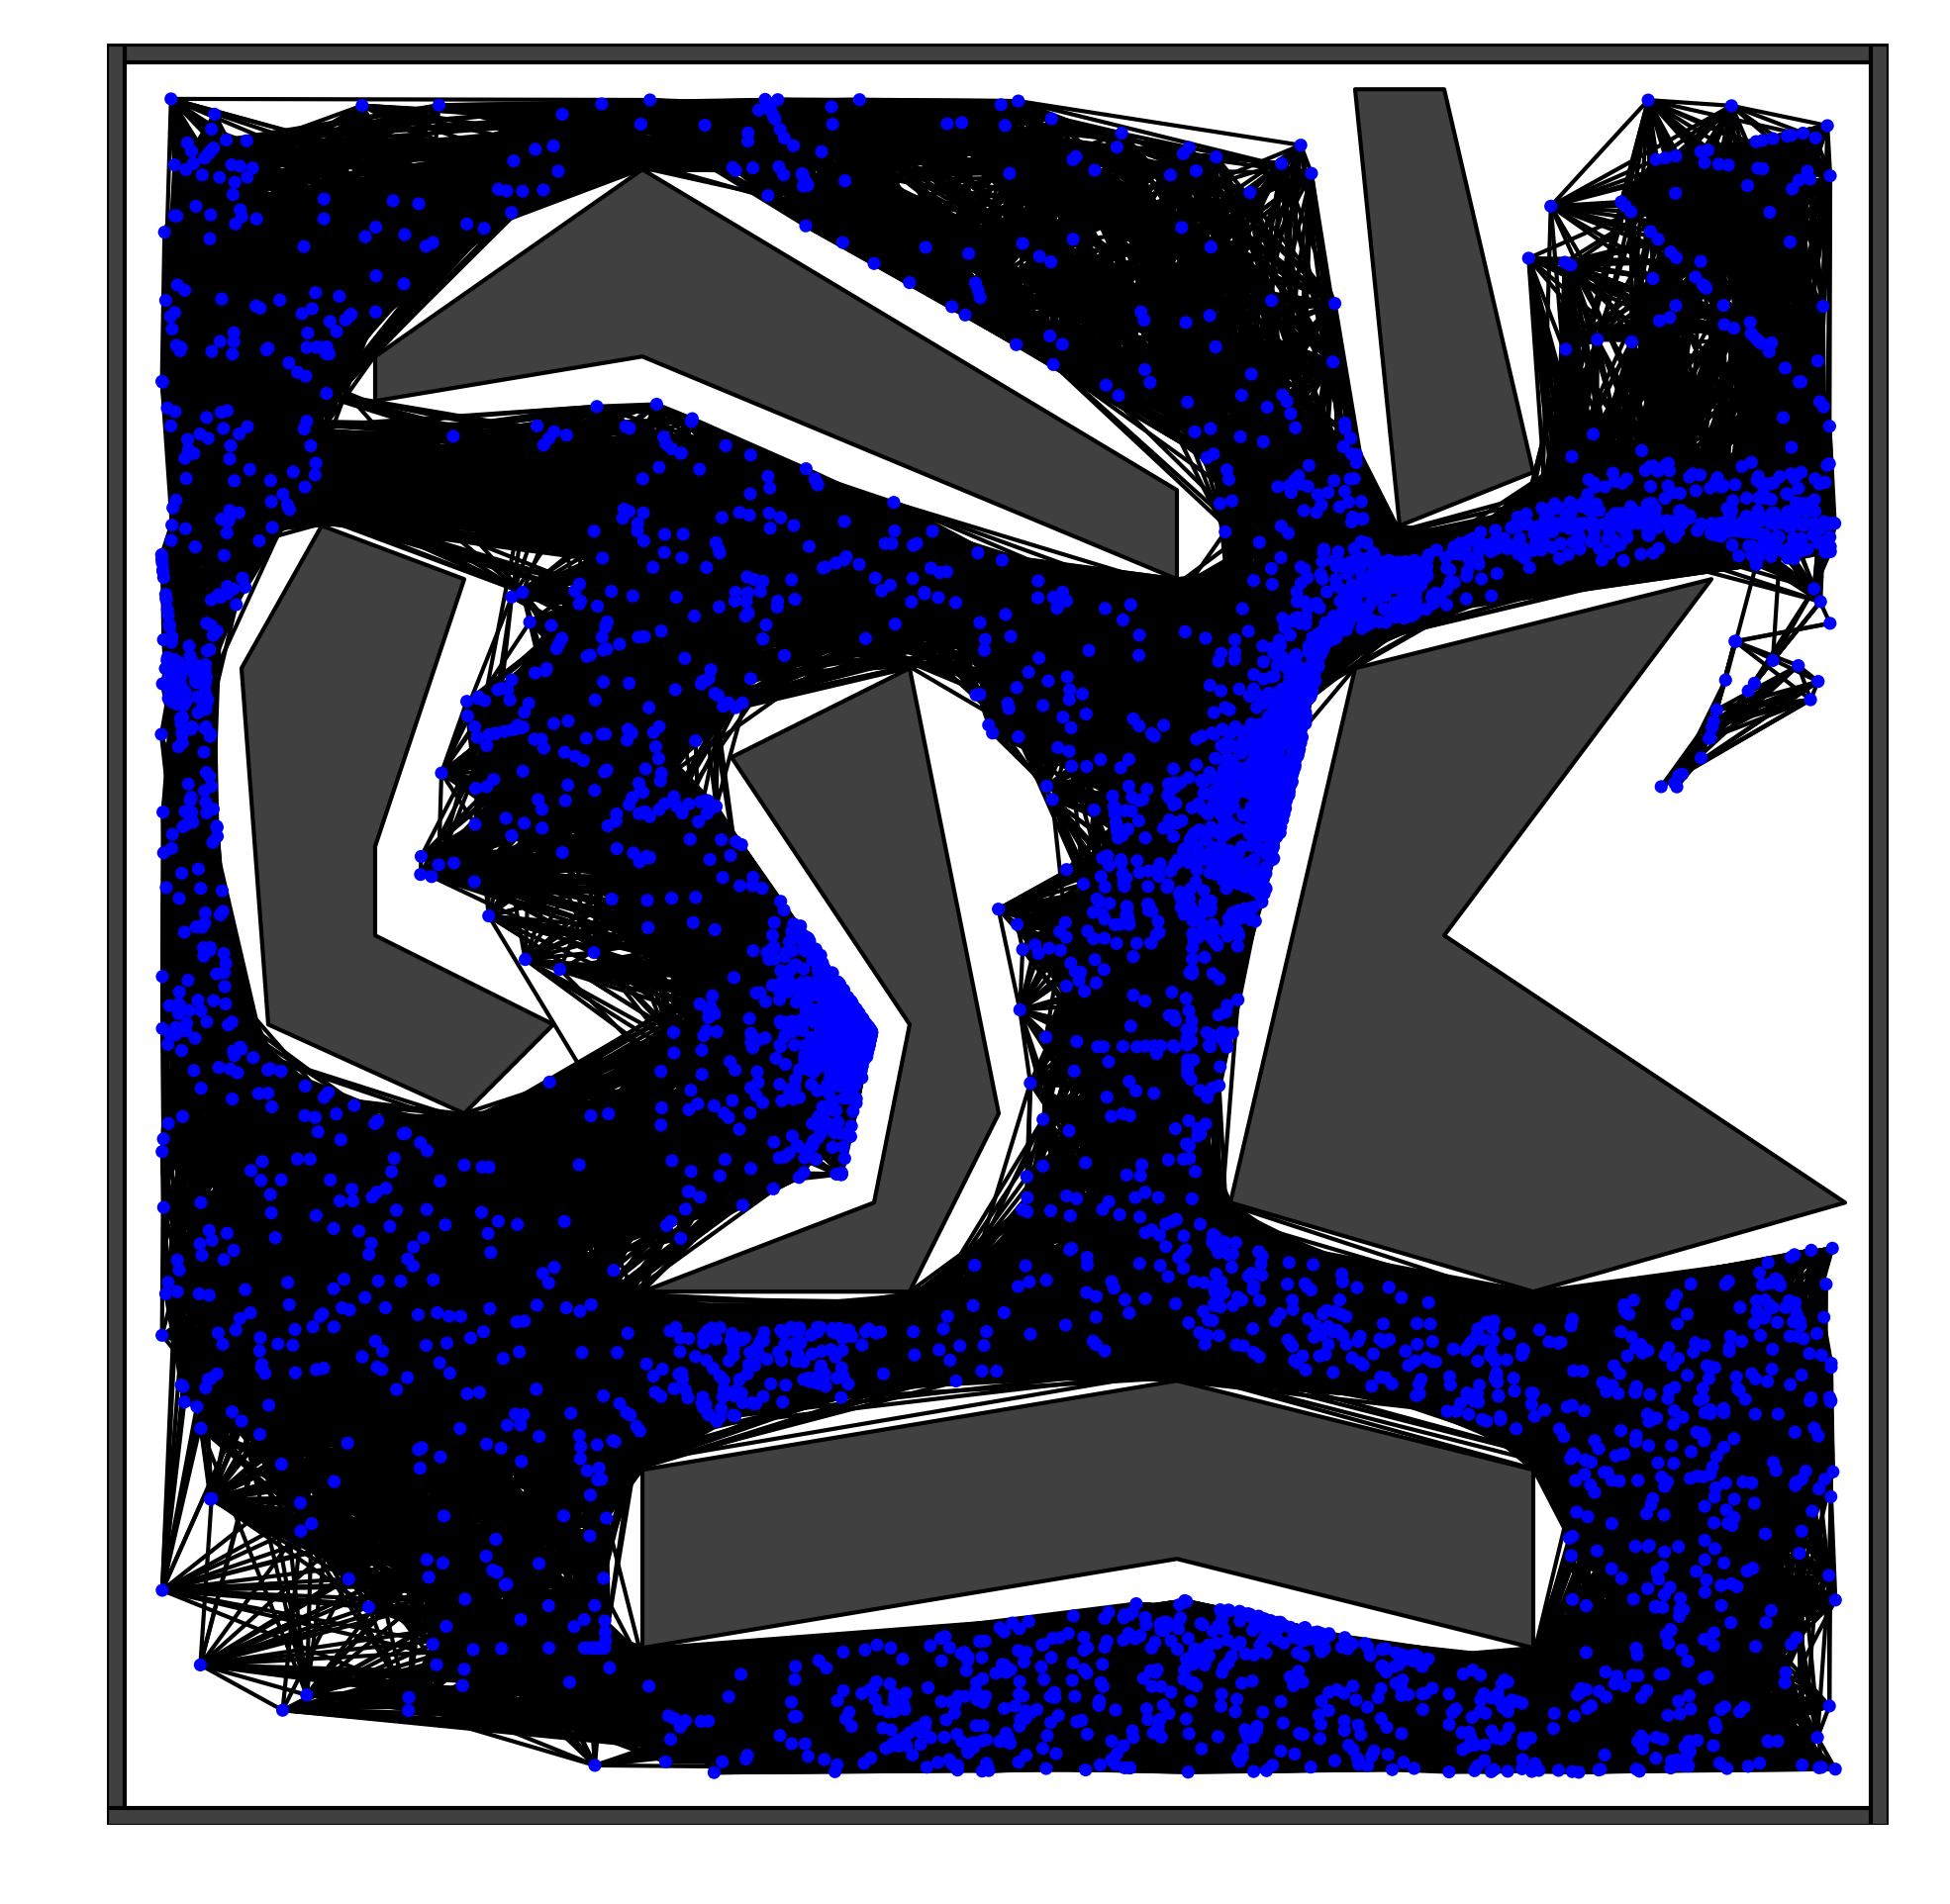
\includegraphics[width=0.325\textwidth]{fig/pinball-graph-pruned.png}\label{fig:pinball-graph-pruning}}%
\subbottom[Graph clustering]{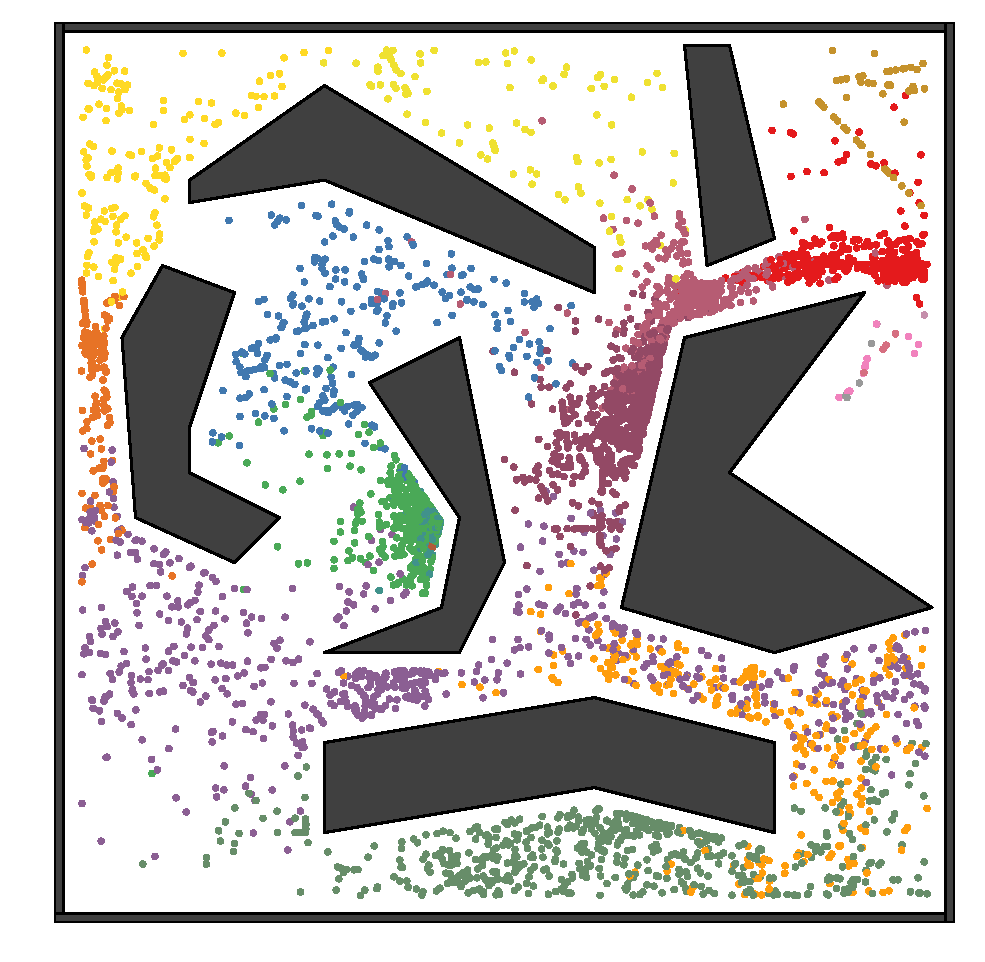
\includegraphics[width=0.32\textwidth]{fig/pinball-clustering.pdf}}
\caption{Pinball domain for reinforcement learning}
\end{figure}

For easier comparison with the results presented in \cite{Konidaris2009}, the obstacles layout named \texttt{pinball\_simple\_single.cfg} from the open source implementation \footnote{\url{http://www-all.cs.umass.edu/~gdk/pinball/}} of the author was used. It has been chosen to implement \footnote{\url{https://github.com/pierrelux/pypinballl}} Pinball in Python rather than using the Java package already made available. One reason for this was to simplify the integration with the Python-RL \footnote{\url{https://github.com/amarack/python-rl}} project from which some components had been used. Great care has however been taken in ensuring that the two implementations behave exactly in the same way. 

\section{Graph Construction}

Instead of collecting samples from a random walk process, a Sarsa($\lambda$) agent was trained with $\alpha = 0.001, \gamma = 0.9, \lambda = 0.9, \epsilon = 0.01$ and 50 trajectories were collected from it. This choice was motivated by the practical need of keeping the number of samples as low as possible and only collect the most relevant ones. The set or trajectories was then merged into one dataset resulting in 48060 sampled states. The dataset was  later uniformly subsampled down to 5000 data points for easier experimentation.

The \texttt{FLANN} library of \cite{Muja2009} was then used to build an approximate nearest neighbors index for the construction of the symmetric KNN graph. The \texttt{igraph} library of \cite{Csardi2006} was used to manipulate the graph more easily. The choice of the number of nearest neighbors $K$ was based on an empirical evaluation and the objective of keeping it as small as possible while minimizing the number of communities found by \textsc{Walktrap} and maximizing the so-called \textit{modularity}. A given graph partitioning among $c$ clusters or \textit{modules} has a high value of modularity when the density of connections within a module is high compared to the inter-module ones. A definition of this measure given by \cite{Newman2006} is

\begin{align}
Q &= \sum_{i}^c \left( e_{ii} - a_i^2 \right) \\
e_{ii} &= \sum_j 	\frac{A_{ij}}{2m} \delta(c_i, c_j) \\
a_i &= \sum_j e_{ij}
\end{align}

The $e_{ii}$ term here above is the fraction of edges within community $i$ while $a_i$ is of those edges with at least one vertex in $i$. \textsc{Walktrap} does not directly optimizes the modularity but rather uses the diffusion-like distance as presented in section \ref{sec:walktrap}.
The vertex dendogram produced by Ward's algorithm is however cut at its maximum of modularity. 

\begin{figure}
\centering
\subbottom[From top to bottom: influence of the number of nearest neighbors on the number of edges, number of communities and modularity. Averaged over 10 graphs for each $K$]{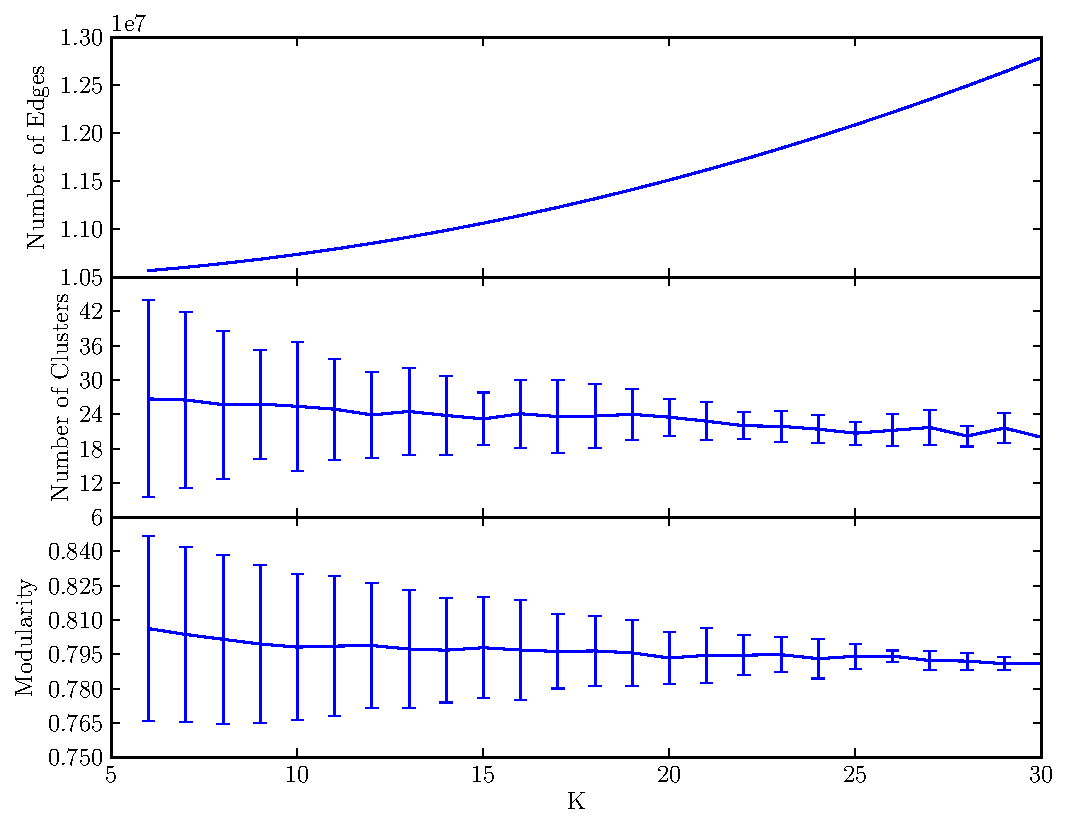
\includegraphics[width=0.49\textwidth]{fig/knn-influence.pdf}\label{fig:knn-vs-clusters}}\hspace{2mm}%
\subbottom[From top to bottom: influence of the number of random walk steps on the number of communities found and associated modularity.]{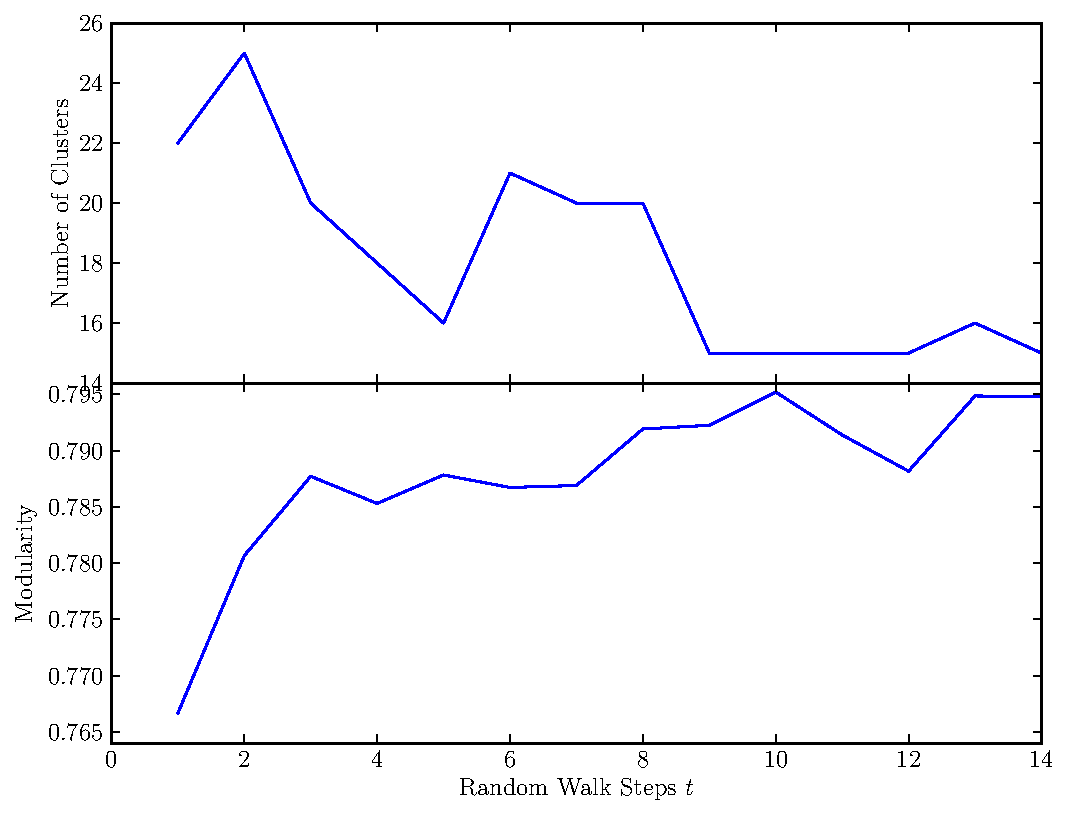
\includegraphics[width=0.49\textwidth]{fig/steps-influence.pdf}\label{fig:steps-vs-clusters}}
\label{fig:pinball-graph}
\caption{Effect of $K$ and $t$ during graph construction and clustering}
\end{figure}

As $K$ increases, the graph becomes denser and drives the communities to be more compact and less numerous. \textsc{Walktrap} being $\mathcal{O}(mn^2)$, higher values of $K$ also have a direct impact on the running time as the number of edges $m$ gets larger. The presence of error bars in figure \ref{fig:knn-vs-clusters} is due to the approximate nearest neighbour graph construction which results in probabilistic edge assignments. As $K$ gets larger, the graph gets denser and the clustering becomes more stable. Intuitively, adding more edges in an already dense graph should have less of an impact on the inter-community transition probabilities than for a very sparse one. A perturbation analysis could shed some light on this phenomenon. Based on the curves shown in figure \ref{fig:knn-graphs}, $K=25$ was retained for this experiment as it yielded good clustering stability and an edge set $|E| = 90348$ of tractable size. 

The number of random walk steps in \textsc{Walktrap} affects the scale at which the dynamical proximity is measured. As discussed in section \ref{sec:walktrap}, the graph density should be considered in this choice. For large values of $K$, the resulting denser graph will blur away faster the difference between pairs of vertices under longer random walks. Figure \ref{fig:steps-vs-clusters} shows this phenomenon starting from $t=8$ where the number of communities sharply decreases from 26 to 16 as the vertices get dynamically more similar. A smaller number of time steps $t=4$ was deemed appropriate for this experiment, providing big enough communities, a modularity of 0.7852 and fast computation.

A post-processing step was added in this experiment in order to prune infeasible edges and improve the graph representation. In the Pinball domain, the observation space leads to a graph representation where edges are set between four-dimensional Euclidean points of the form $[x, y, \dot{x}, \dot{y}]$. While it can be difficult to establish the feasibility of a transition between any two such points, it is clear that no edge should cross the obstacles in the x-y plane. A line intersection test is thus performed over the symmetric graph to remove any such edge (figure \ref{fig:pinball-graph-pruning}). The options construction algorithm can be dispensed with this step in the absence of such domain specific knowledge. The experience has however shown that it can greatly improve the clustering quality.

\section{Learning}

\begin{figure}
\centering
\subbottom[The flat policy take more episodes to achieve the same number of steps as the one over options]{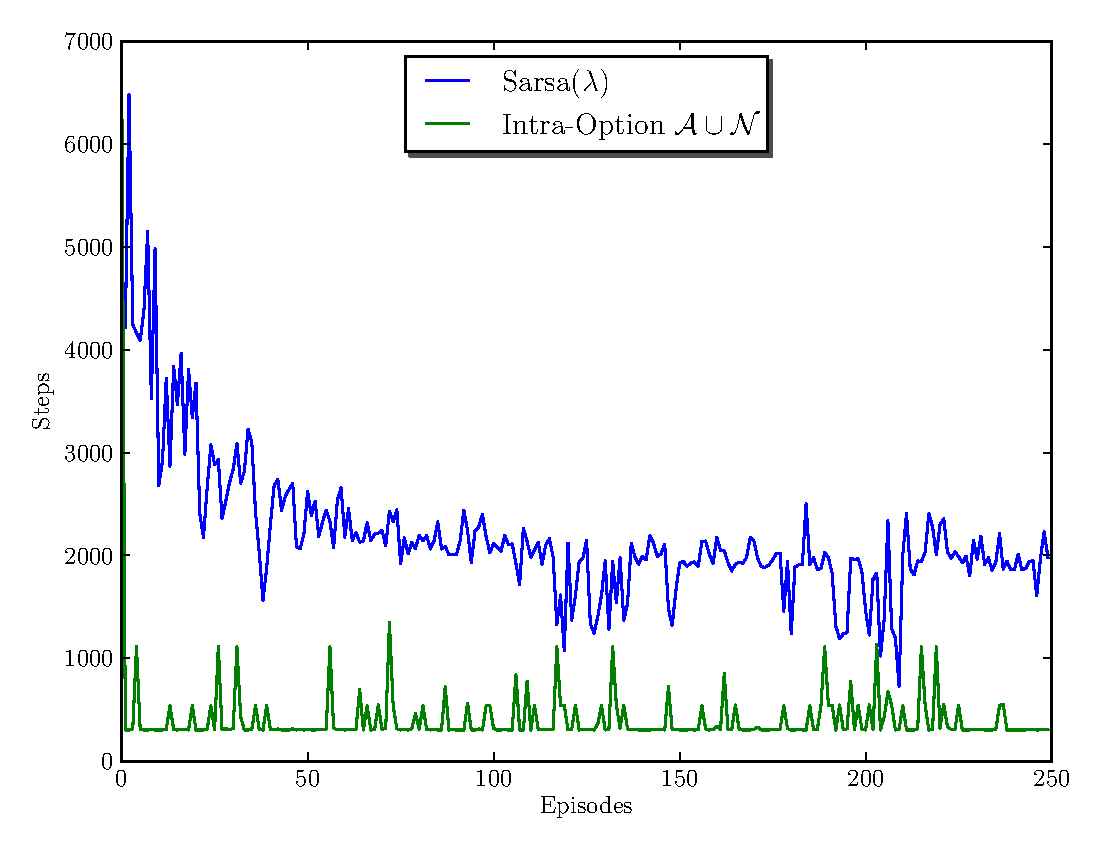
\includegraphics[width=0.49\textwidth]{fig/sarsa-intra.eps}}\hspace{2mm}%
\subbottom[Bottleneck options produce uncontrollable oscillatory behavior at the boundary]{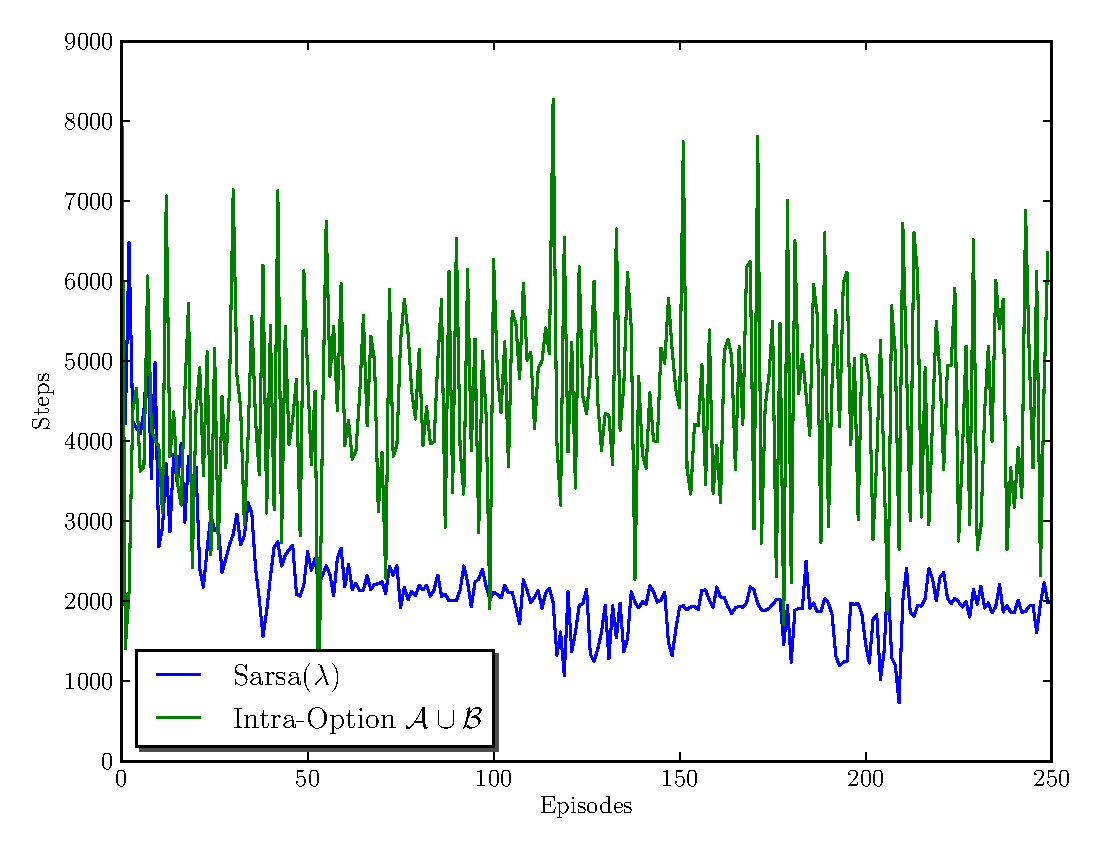
\includegraphics[width=0.49\textwidth]{fig/pinball-bottleneck.eps}\label{fig:pinball-bottleneck}}
\caption{Learning with options}
\end{figure}

The bottleneck options algorithm \ref{alg:knnoptions} was applied over the clustering for the definition of the initiation, policy and termination components of the options. The bottleneck construction seeks option policies which can bring the agent at the boundary of their respective cluster from any state within the initiation set. It was found however that the \textit{vanilla} bottleneck concept appears to be flawed when it comes to the continuous case. The canonical HRL domain for motivating the bottleneck concept has been mainly concerned with the \textit{doors and rooms} domains in discrete state space. In an environment such as the four-rooms domain \parencite{Sutton1999}, bottlenecks are precisely those single rectangular cells connecting two rooms in the x-y plane. 

The situation becomes much more complex for the type of community structures found in Pinball. The problem is twofold: the number of adjacent communities is larger and the bottleneck regions are wider. The difficulty stems mostly from the fact that bottlenecks are now identified in a four-dimensional space rather than only across x-y coordinates. In the four-rooms domain, learning a policy which bring the agent to any of its two doors arbitrarily at random would not impact the rate of convergence as much. The agent should however be constrained to an optimal stochastic choice about which of the bottleneck states should be reached in order to obtain maximum payoff. Furthermore, as the number of adjacent communities gets larger, the number of possible outcomes arising from a transition to any of them might increase and become difficult to evaluate. This intuition was verified empirically by training the bottleneck options using the Sarsa($\lambda = 0.9$) algorithm with learning rate $\alpha = 0.001$, discount factor $\gamma = 0.9$ and an epsilon-greedy exploration strategy with $\epsilon = 0.01$. A policy over such options was then obtained using \textsc{Intra-Option Learning} with $\alpha = 0.001, \gamma = 0.9, \epsilon = 0.01$. A linear fourth-order Fourier approximation of the action-value function was used for every flat or options-based agent. Figure \ref{fig:pinball-bottleneck} compares the number of steps taken per episode with that of a flat Sarsa($\lambda$) learning agent. The latter shows steady convergence to some successful policy which can take the ball from its initial position to the goal. No learning however seems possible under the naive bottleneck construction and intra-option learning is very unstable. 

\section{Navigation Options}

The need to impose a stochastic choice on which bottlenecks to reach on the boundary leads to slightly different kind of options referred to as \textit{navigation options} in this thesis. This designation highlights the fact that such options specify policies to \textit{navigate} between fixed pairs of adjacent communities.

\begin{algorithm}
\DontPrintSemicolon
\KwData{An environment from which to collect experience, terminal subgoal reward $R_{subgoal}$, number of random walk steps $t$, number of nearest neighbors $k$}
\KwResult{A set of options}
\SetKwData{Dataset}{dataset}
\SetKwData{Index}{index}
\SetKwData{Edges}{edges}
\SetKwData{Vertices}{vertices}
\SetKwFunction{Walktrap}{Walktrap}
\SetKwData{g}{g}
\SetKwFunction{Graph}{Graph}
\SetKwData{Communities}{communities}
\SetKwFunction{Option}{Option}
\SetKwData{Options}{options}
\SetKwData{Subgoals}{subgoals}
\SetKwFunction{Boundary}{$\partial$}
\SetKwFunction{LearnMDP}{LearnSubgoalMDP}
\SetKwFunction{Mode}{Mode}
\SetKwData{Adjacencies}{adjacencies}
\SetKwData{ModeLabel}{label}
\SetKwData{ModeFreq}{frequency}
\SetKwData{KNN}{knn}
\SetKwData{Membership}{membership}
\SetKwData{Label}{label}
\SetKwData{AdjLabel}{adjLabel}
\;

\textbf{1. Acquire experience} \;
\textbf{2. Build the symmetric K-NN graph}\;
\textbf{3. Discover and learn options} \;
\textbf{3.1 Establish relevant adjacent communities}\;
\Communities, \Membership $\leftarrow$ \Walktrap{\Graph{\Vertices, \Edges}, t} \;
\Adjacencies $\leftarrow \underbrace{[ \varnothing, \dots, \varnothing]}_{|\Communities|}$\;
\ForEach{community c \KwSty{in} \Communities} {
  \ForEach{node n \KwSty{in} c} {
     \KNN $\leftarrow$ query the $k$ nearest neighbors of $n$\;
     \ModeLabel, \ModeFreq $\leftarrow$ \Mode{\KNN} \;
     \If{\DataSty{label} $\not =$ \DataSty{membership[n]} \KwSty{and} \DataSty{frequency} $\geq \lceil \frac{k}{2} \rceil$} {
        $\Adjacencies[\Membership[n]] \leftarrow \Adjacencies[\Membership[n]] \cup \Label$\;
      }
    }
}
\textbf{3.2 Learn options}\;
\Options $\leftarrow \varnothing$ \;
\ForEach{$\langle \Label , \AdjLabel \rangle$ \KwSty{in} \Adjacencies} {
  $\mathcal{I} \leftarrow \Communities[\Label]$\;
  $\Subgoals \leftarrow \Communities[\AdjLabel]$\;
  $\beta \leftarrow \indicator_{\Subgoals}$ \;
   $\g \leftarrow \indicator_{\Subgoals}\cdot R_{subgoal}$\;
   $\pi \leftarrow$ \LearnMDP{\g} \;
   \Options $\leftarrow$ \Options $\; \cup \;$ \Option{$\mathcal{I}$, $\beta$, $\pi$} \;
}

\Return \Options
\caption{\textsc{Navigation-Options} construction algorithm}
\label{alg:navoption}
\end{algorithm}

Algorithm \ref{alg:navoption} is identical to \ref{alg:knnoptions} on the sampling and graph construction steps. It however differs in the option discovery and construction approach by defining options \textit{between} communities. The adjacent communities could be discovered simply by considering the bottleneck edges and the label of their adjacent vertices. While this approach would be valid in a perfect graph representation, the identification of relevant bottleneck states is hindered by the high edge density need for clustering. Under such densities, most vertices of a community are also bottleneck states. It is thus desirable to identify adjacent communities on the basis of a sparser proximity graph. Algorithm \ref{alg:navoption} for navigation options thus queries the $k$ nearest neighbors and the most frequent label appearing among them is subject to majority test before establishing the adjacency relation. This procedure both reduces the number bottleneck outliers and irrelevant adjacent communities.

\begin{figure}
\centering
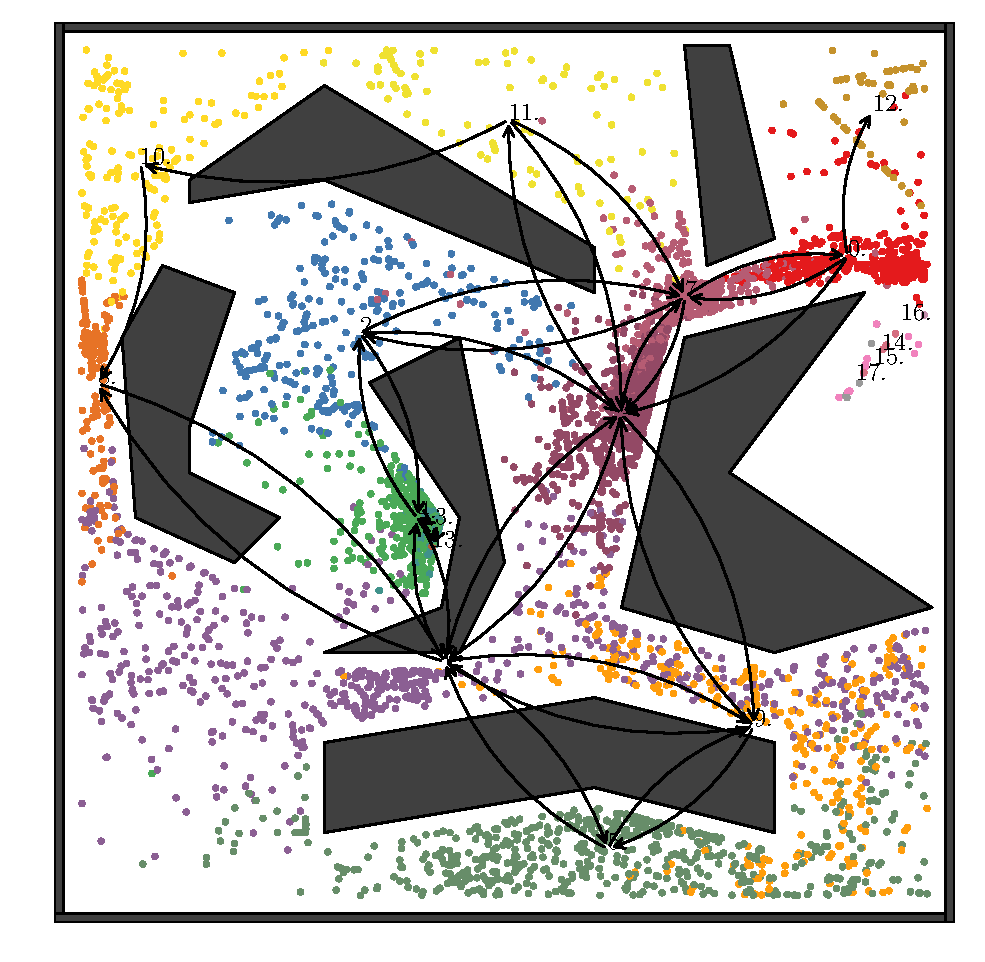
\includegraphics[width=0.49\textwidth]{fig/pinball-nav.pdf}
\caption{Navigation options found using algorithm \ref{alg:navoption}. Each arrow corresponds to an option for transitioning across the given pair of communities. Macro transitions 1 to 7, 5 to 6, 6 to 1, and 7 to 0 were manually selected for learning.}
\label{fig:nav-options}
\end{figure}

The navigation options construction was applied over the 18 communities found by \textsc{Walktrap} at maximum modularity under $t=4$. It lead to 34 adjacency relations being established, pruning at the same time small communities consisting of only a few vertices. The learning curve in figure \ref{fig:nav-options} was obtained by averaging 10 \textsc{Intra-Option} learning agents with $\alpha = 0.1, \gamma = 0.9, \epsilon = 0.1$ and a fourth order Fourier approximation. 

The off-policy \textsc{Intra-Option Learning} is known to diverge under function approximation. Such a problem was encountered during experimentation and motivated the decision to manually select a subset of four options from the 34 found automatically. Such a simplification reduced the learning complexity and made the task of finding suitable learning parameters more easy. The options set used in \ref{fig:nav-options} thus consisted of the five primitive actions of pinball augmented with these four navigation options. From the very few first episodes, it can be seen that the agent having access to options successfully learnt to reach the target under approximately 300 steps while the Sarsa agent having access to only primitive actions flattens off above 1000. 

%\begin{figure}
%\centering
%\subbottom[Intra-Option learning can diverge with function approximation]{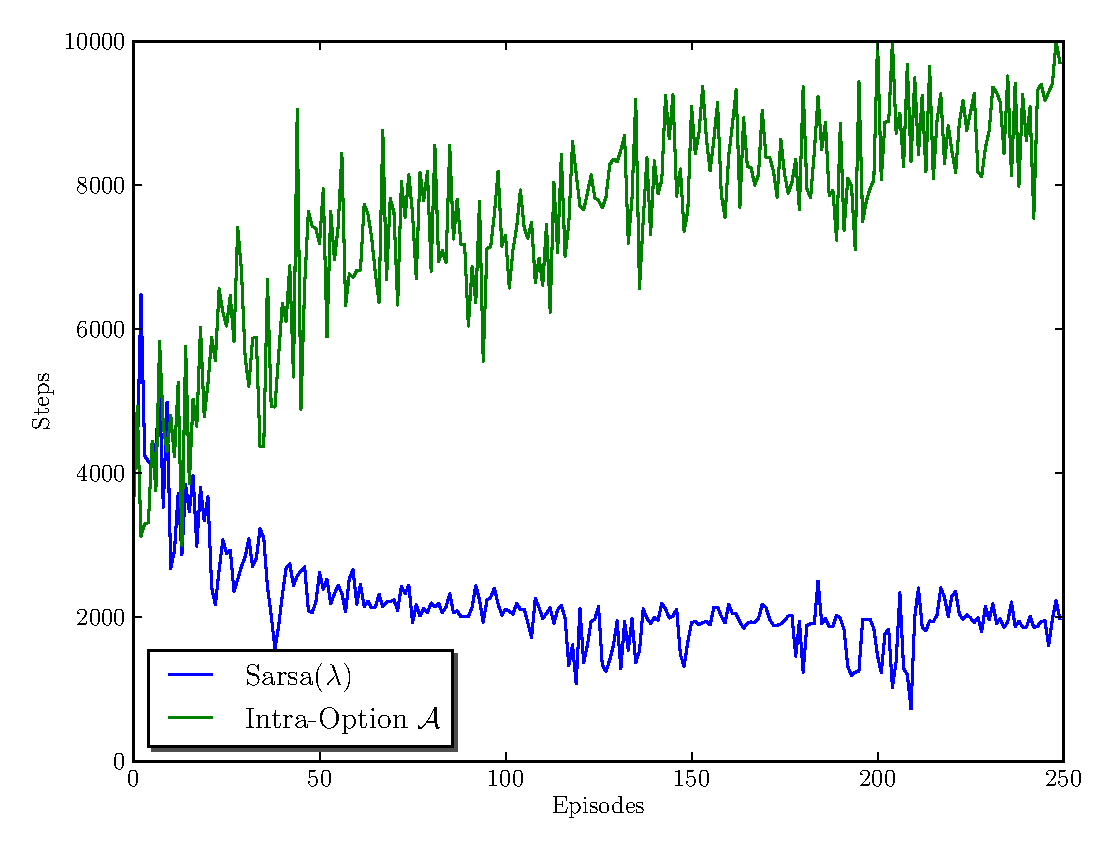
\includegraphics[width=0.49\textwidth]{fig/intra-diverge.eps}}
%\end{figure}